\documentclass[12pt,a4paper]{article}
\usepackage[utf8]{inputenc}
\usepackage{amsmath,amssymb,amsfonts,amsthm}
\usepackage{geometry}
\usepackage{enumitem}
\usepackage{fancyhdr}
\usepackage{lastpage}
\usepackage{graphicx}

% Page layout
\geometry{margin=1in}
\pagestyle{fancy}
\fancyhf{}
\lhead{Lucas Cassin Cruz Burke}
\rhead{AMATH 563}
\rfoot{Page \thepage\ of \pageref{LastPage}}

% Theorem environments
\theoremstyle{definition}
\newtheorem{problem}{Problem}
\theoremstyle{remark}
\newtheorem*{solution}{Solution}

\title{AMATH 563 Homework 2}
\author{Lucas Cassin Cruz Burke}
\date{April 28, 2023}

\begin{document}

\maketitle

\section{Theory}

\begin{problem}
    Suppose $\Gamma : \mathcal X \times \mathcal X \rightarrow \mathbb R$ is a PDS kernel. Prove that $\forall x, x' \in \mathcal X$ it holds that $|\Gamma(x,x')|^2 \le \Gamma(x,x) \Gamma(x',x')$. 
\end{problem}
\begin{solution}
    To prove this, consider the 2-by-2 kernel matrix $$\begin{bmatrix}
        \Gamma(x,x) & \Gamma(x,x') \\
        \Gamma(x',x) & \Gamma(x',x')
    \end{bmatrix}$$

    Since $\Gamma$ is a PDS kernel, the matrix $K$ is positive semi-definite. Therefore, all of its principal minors, including its determinant, must be non-negative, hence we have $$\Gamma(x,x)\Gamma(x',x') - \Gamma(x,x')\Gamma(x',x) \ge 0$$

    Since $\Gamma$ is a symmetric kernel (as are all PDS kernels), we have $\Gamma(x,x') = \Gamma(x',x)$, and so this inequality becomes $$\Gamma(x,x) \Gamma(x',x') - |\Gamma(x,x')|^2 \ge 0$$

    Rearranging, we get our result 

    $$|\Gamma(x,x')|^2 \le \Gamma(x,x)\Gamma(x',x')$$
\end{solution}

\begin{problem}
    Given a kernel $K$ on $\mathcal X$ define its normalized version as $$\bar K(x,x') = \begin{cases}
        0 & \text{if $K(x,x)=0$ or $K(x',x')=0$} \\
        \frac{K(x,x')}{\sqrt{K(x,x)}\sqrt{K(x',x')}} & \text{Otherwise}
    \end{cases}$$

    Show that if $K$ is PDS then so is $\bar K$. 
\end{problem}
\begin{solution}
    We need to show that for any $X={x_1, \dots, x_n} \subset \mathcal X$ and any $\xi \in \mathbb R^n$, we have $\xi^T \bar{K}(X,X) \xi \ge 0$.

    First, note that if $K(x_i, x_i) = 0$ or $K(x_j, x_j) = 0$ for any $i, j$, then $\bar{K}(x_i, x_j) = 0$, and $\xi^T \bar{K}(X,X) \xi = 0 \ge 0$. 

    Otherwise, we have $$\xi^T \bar{K}(X,X) \xi = \sum_{i=1}^n \sum_{j=1}^n \xi_i \xi_j \frac{K(x_i,x_j)}{\sqrt{K(x_i,x_i)}\sqrt{K(x_j,x_j)}}$$

    Now let us define $\eta_i = \frac{\xi_i}{\sqrt{K(x_i, x_i)}}$ and $\eta_j = \frac{\xi_j}{\sqrt{K(x_j,x_j)}}$. With these new variables our expression becomes $$\sum_{i=1}^n \sum_{j=1}^n \eta_i \eta_j K(x_i,x_j) \ge 0$$

    Where the inequality comes from the fact that $K$ is PDS. Therefore we conclude that $\bar K$ is likewise PDS whenever $K$ is PDS. 
\end{solution}

\begin{problem}
    Show that the following kernels on $\mathbb R^d$ are PDS: 
    \begin{itemize}
        \item Polynomial kernel: $K(x,x') = \left( x^T x' + c \right)^\alpha$ for $c>0$ and $\alpha \in \mathbb N$. 
        \begin{solution}
            We note that $K^{(0)}(x,x') = x^Tx'$ on $\mathbb R^d$ is the linear kernel, which we know to be PDS, as it is the Euclidian dot product. From this it follows that $K^{(1)}(x,x') = K^{(0)}(x,x') +c = x^T x' + c$ is also PDS, since $c >0$ and the sum of PDS kernels is PDS. Lastly, since the product of PDS kernels is PDS, we have that $K(x,x') = (K^{(1)}(x,x'))^{\alpha} = \left( x^T x' + c \right)^\alpha$ is PDS. Hence the polynomial kernel is PDS. 
        \end{solution}
        \item Exponential kernel: $K(x,x') = \exp(x^T x')$. 
        \begin{solution}
            We note that $K(x,x') = \exp(K^{(0)}(x,x'))$, where $K^{(0)}(x,x') = x^T x'$ is the linear kernel, which we know to be PDS. Then we have $$K(x,x') = \exp(K^{(0)}(x,x')) = \sum_{n=0}^\infty \frac{\left(K^{(0)}(x,x')\right)^n}{n!} = \lim_{N\rightarrow \infty} \sum_{n=0}^N \frac{\left(K^{(0)}(x,x')\right)^n}{n!}$$

            First, we recognize that each $\left(K^{(0)}(x,x')\right)^n$ term is PDS, since $\left(K^{(0)}(x,x')\right)^n$ is the product of $n$ PDS kernels and the product of PDS kernels is PDS. Next we note that each partial sum $\sum_{n=0}^N \frac{\left(K^{(0)}(x,x')\right)^n}{n!}$ is also PDS, since it is the weighted sum of $n$ PDS kernels, and the weighted sum of PDS kernels is PDS. Hence, we see that $K(x,x')$ is the limit of a sequence of PDS kernels. Since the limit of a sequence of PDS kernels is PDS whenever said limit exists, it follows that $K(x,x')$ is also PDS. Hence the exponenetial kernel is PDS.
        \end{solution}
        \item RBF kernel: $K(x,x') = \exp (-\gamma^2 ||x-x'||_2^2)$.
        \begin{solution}
            We have 

            \begin{align*}
                K(x,x') &= \exp(-\gamma^2 ||x-x'||_2^2) = \exp\left(-\gamma^2(||x||^2 - 2 \langle x, x' \rangle + ||x'||^2)\right) \\
                &= \exp\left(-\gamma^2(||x||^2 + ||x'||^2)\right) \exp \left( 2 \gamma^2 \langle x, x' \rangle \right)
            \end{align*}

            Let us define $K_1(x,x') = \exp\left(-\gamma^2(||x||^2 + ||x'||^2)\right)$ and $K_2(x,x') = \exp \left( 2 \gamma^2 \langle x, x' \rangle \right)$. Note that since $\langle x, x' \rangle$ is an inner product we know that it is PDS, therefore since $K_2$ is the exponential of a PDS kernel it is also a PDS kernel. (See PDS proof for exponential kernels above). 

            Now consider any $X = \{x_1, \dots, x_m \} \subset \Omega$ and any $\xi \in \mathbb R^m$. For the $K_1$ kernel we have
            
            \begin{align*}
                \xi^T K_1(X,X) \xi &= \sum_{i=1}^m \sum_{j=1}^m \xi_i \xi_j K_1(x_i, x_j) = \sum_{i=1}^m \sum_{j=1}^m \xi_i \xi_j \exp\left(-\gamma^2(||x_i||^2 + ||x_j||^2)\right) \\
                &= \left( \sum_{i=1}^m \xi_i \exp\left(-\gamma^2||x_i||^2 \right) \right)^2 \ge 0
            \end{align*}

            Hence $K_1$ is also PDS. Therefore $K(x,x') = K_1(x,x')K_2(x,x')$ is the product of two PDS kernels, and hence it must likewise be PDS.  
        \end{solution}
    \end{itemize}
\end{problem}

\begin{problem}
    Let $\Omega \subseteq \mathbb R^d$ and let $\{\psi_j\}_{j=1}^n$ be a sequence of continuous functions on $\Omega$ and $\{\lambda_j\}_{j=1}^n$ a sequence of non-negative numbers. Show that $K(x,x')=\sum_{j=1}^n \lambda_j \psi_j(x) \psi_j(x')$ is a PDS kernel on $\Omega$. 
\end{problem}
\begin{solution}
    First, let us define $K_j(x,x') = \psi_j(x)\psi_j(x')$, so that $K(x,x') = \sum_{j=1}^n \lambda_j K_j(x,x')$. Each $K_j$ forms a PDS kernel, since for any $X=\{x_1,\dots, x_m\} \subset \Omega$ and any $\xi \in \mathbb R^m$ we have $$\xi^T K_j(X,X)\xi =\sum_{i=1}^m \sum_{k=1}^m \xi_i \xi_k \psi_j(x_i)\psi_j(x_k) = \left(\sum_{i=1}^m \xi_i \psi_j(x_i) \right)^2 \ge 0$$ 

    Now, we observe that the kernel $K(x, x')$ is a linear combination of the $K_j(x, x')$ with non-negative coefficients $\lambda_j$. It is a well-known fact that a linear combination of PDS kernels with non-negative coefficients is also a PDS kernel. Therefore, $K(x, x')$ is a PDS kernel.
\end{solution}

\begin{problem}
    Show that: (i) if $K$ and $K'$ are two reproducing kernels for an RKHS $\mathcal H$, then they have to be the same. (ii) the RKHS of a PDS kernel $K$ is unique.
\end{problem}
\begin{solution}
    First, we will show that if $K$ and $K'$ are two reproducing kernels for an RKHS $\mathcal H$, then they must be the same. 

    Let $x \in \mathcal X$. We have that for all $f \in \mathcal H$, $$f(x) = \langle f, K(x, \cdot) \rangle = \langle f, K'(x, \cdot) \rangle$$

    Since this holds for all $f \in \mathcal H$, by the Riesz representation theorem, we have that $K(\cdot, x) = K'(\cdot, x)$. Because this holds for all $x \in \mathcal X$, we conclude that $K = K'$.

    Next, let us show that the RKHS of a PDS kernel $K$ is unique. 

    Let $\mathcal H$ and $\mathcal H'$ be two RKHSs of a PDS kernel $K$. Then $K$ is a reproducing kernel for both $\mathcal H$ and $\mathcal H'$. From part (i), we know that any two reproducing kernels for an RKHS have to be the same. Therefore, the reproducing kernels of $\mathcal H$ and $\mathcal H'$ are the same, so they induce the same inner product and norm on their respective function spaces.

    Because $\mathcal H$ and $\mathcal H'$ have the same inner product and norm, they are isometrically isomorphic as Hilbert spaces. Therefore, the RKHS of a PDS kernel $K$ is unique up to isometric isomorphism.
\end{solution}

\section{Computation}

In this section we will use kernel regression techniques to train digit classifiers using the famous MNIST dataset of 28x28 handwritten digits. We create a total of four classifiers, which are able to distinguish between the digit pairs (1,9), (3, 8), (1,7), and (2, 5). 

To reduce the number of input dimensions, we use Principle Component Analysis on the training set. After applying PCA to our full dataset we find that we are able to capture 95\% of the dataset variance using only 331 features. See Figure 1 for a plot of how the variance changes with the number of PCA components.

\begin{figure}[h]
    \centering
    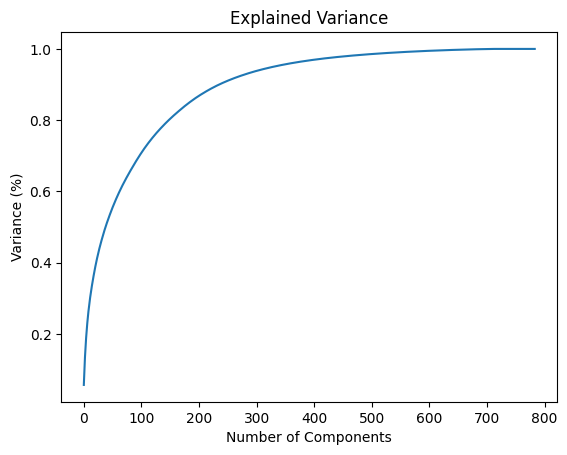
\includegraphics{PCA_Var.png}
    \caption{Plot showing the explained variance of the MNIST dataset as a function of the number of PCA components.}
    \label{fig:fig1}
\end{figure}


In practice will be able to reduce this number even further, as in this assignment we will focus only on distinguishing between two classes of digits, and will therefore be able to discard features which are not relevant to the pair in question. 

The process is as follows. For each digit pair we will create a training and testing dataset using the provided MNIST data. We standardize the features for both datasets by subtracting the mean and dividing by the standard deviation of the training samples. Lastly, we replace the smaller number labels with $-1$ and the larger number labels with $1$ (this had a noticeable impact on accuracy in my experiments). Following this, we use PCA to reduce the number of input components, keeping only as many features as required to preserve 95\% of the training set variance. 

Having normalized our data in each case, we examine the performance of three kernels: RBF, polynomial, and linear. We use sklearn's "GridSearchCV" to perform a cross-validated exhaustive grid-search over a parameter grid, using the following parameter values:

\begin{itemize}
    \item RBF: $\alpha \in \{0.1, 0.5, 1\}$, $\gamma \in \{0.001, 0.01, 0.1, 1\}$
    \item Polynomial: $\alpha \in \{0.1, 0.5, 1\}$, $\text{Degree} \in \{2, 3, 4\}$. 
    \item Linear: $\alpha \in \{0.1, 0.5, 1\}$
\end{itemize}

The prediction error shown corresponds to the percentage of incorrect classifications. 

It was quite interesting to see how certain kernels performed better or worse depending on the digit classes in question. The polynomial and RBF kernels performed better across the board than the linear kernel, and in most cases had roughly similar performance. Interestingly in the 2v5 case the polynomial was nearly an order of magnitude more effective on the test data than the RBF kernel. Perhaps even more strange is that in the 1v9 classification they had the \textit{exact} same performance. I haven't yet ascertained the reason behind this, but it's an interesting result which I'd like to follow up on. In a couple of cases the RBF and/or polynomial kernel achieved 0\% error on the test data. In some of these it seems this may have led to overfitting and the kernel underperformed its competitors, but in others, e.g. polynomial kernel in the 2v5 classification, it seemed to indicate a genuinely high degree of accuracy which carried over into the test set. 

Overall I came away impressed with the effectiveness of this method. I'd like to see how this performance changes when dealing with the full 9-digit classification problem. Additionally, I'd be curious to see how the training efficiency compares with other methods. In my experiments the kernel regression took a little over 10 minutes in most cases on my machine (M1 Macbook Air). This would obviously be slower had I used a more fine-grain parameter grid, however even with a fairly sparse set of parameter values the method was quite accurate. 

\subsection{1 vs. 9 classification}
\subsubsection{RBF kernel}
\begin{itemize}
    \item Best parameters: $\alpha = 0.1$ and $\gamma = 0.001$. 
    \item Training error: 0.000709
    \item Test error: 0.004197
\end{itemize}

\subsubsection{Polynomial kernel}
\begin{itemize}
    \item Best parameters: $\alpha = 1$ and $\text{Degree} = 2$. 
    \item Training error: 0.000709
    \item Test error: 0.004197
\end{itemize}

\subsubsection{Linear kernel}
\begin{itemize}
    \item Best parameters: $\alpha = 1$. 
    \item Training error: 0.004018
    \item Test error: 0.006996
\end{itemize}

\subsection{3 vs. 8 classification}
\subsubsection{RBF kernel}
\begin{itemize}
    \item Best parameters: $\alpha = 0.1$ and $\gamma = 0.001$. 
    \item Training error: 0.000834
    \item Test error: 0.007056
\end{itemize}

\subsubsection{Polynomial kernel}
\begin{itemize}
    \item Best parameters: $\alpha = 1$ and $\text{Degree} = 3$. 
    \item Training error: 0.000000
    \item Test error: 0.003528
\end{itemize}

\subsubsection{Linear kernel}
\begin{itemize}
    \item Best parameters: $\alpha = 1$. 
    \item Training error: 0.035636
    \item Test error: 0.040322
\end{itemize}

\subsection{1 vs. 7 classification}
\subsubsection{RBF kernel}
\begin{itemize}
    \item Best parameters: $\alpha = 0.1$ and $\gamma = 0.001$. 
    \item Training error: 0.001153
    \item Test error: 0.004623
\end{itemize}

\subsubsection{Polynomial kernel}
\begin{itemize}
    \item Best parameters: $\alpha = 1$ and $\text{Degree} = 2$. 
    \item Training error: 0.001537
    \item Test error: 0.006934
\end{itemize}

\subsubsection{Linear kernel}
\begin{itemize}
    \item Best parameters: $\alpha = 1$. 
    \item Training error: 0.006611
    \item Test error: 0.010633
\end{itemize}

\subsection{2 vs. 5 classification}
\subsubsection{RBF kernel}
\begin{itemize}
    \item Best parameters: $\alpha = 0.1$ and $\gamma = 0.001$. 
    \item Training error: 0.000000
    \item Test error: 0.003118
\end{itemize}

\subsubsection{Polynomial kernel}
\begin{itemize}
    \item Best parameters: $\alpha = 1$ and $\text{Degree} = 3$. 
    \item Training error: 0.000000
    \item Test error: 0.000519
\end{itemize}

\subsubsection{Linear kernel}
\begin{itemize}
    \item Best parameters: $\alpha = 1$. 
    \item Training error: 0.020476
    \item Test error: 0.018711
\end{itemize}

\end{document}
